\documentclass{fkssolpub}

\usepackage[czech]{babel}
\usepackage{fontspec}
\usepackage{fkssugar}
\usepackage{amsmath}
\usepackage{graphicx}

\author{Ondřej Sedláček}
\school{Gymnázium Oty Pavla} 
\series{4j}
\problem{3} 

\begin{document}

\section{Část a}

\begin{figure}[h!]
	\begin{center}
		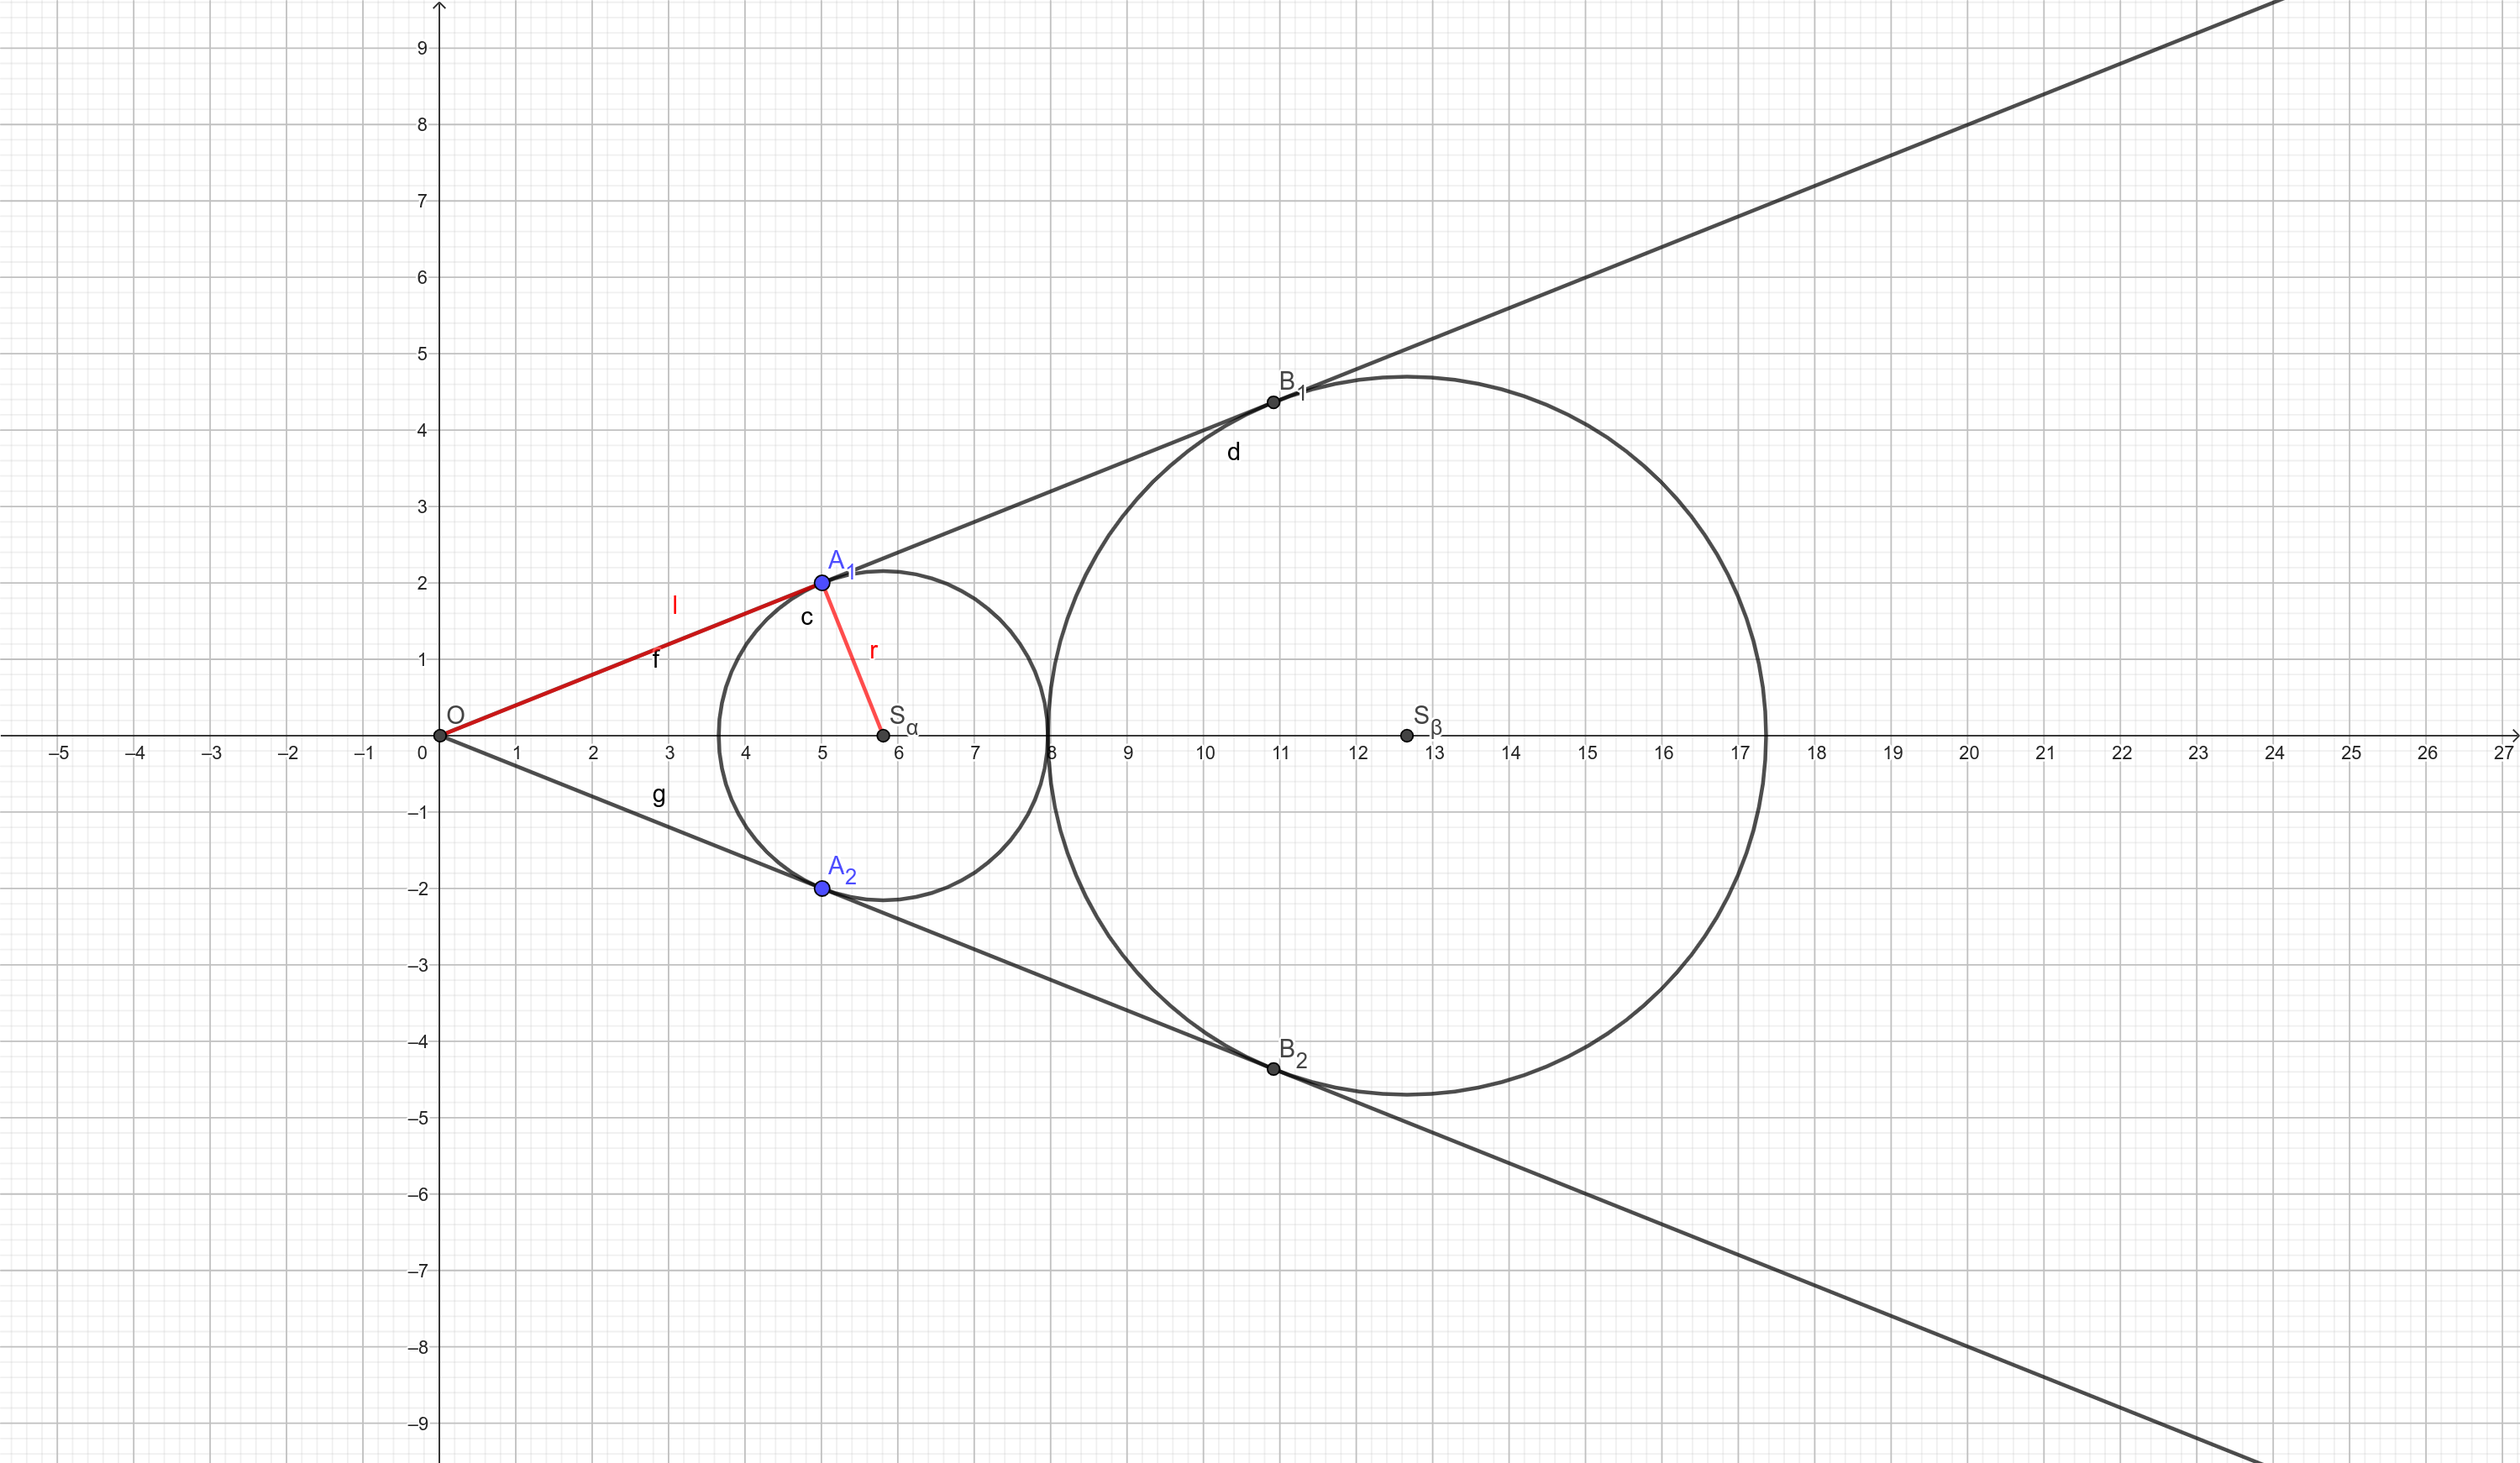
\includegraphics[width=0.95\textwidth]{3-fig.png}
	\end{center}
	\caption{Konstrukce}
	\label{fig:}
\end{figure}


Označme vzdálenost od vrcholu úhlu $O$ od dotykového bodu $A_1$ jako $l$,
poloměr jako $r$ a střed kružnice $\alpha$ jako $S_{\alpha}$. Víme, že
trojúhelník $A_1 O S_{\alpha}$ je pravoúhlý. Tím pádem vzdálenost
$|OS_{\alpha}| = \sqrt{l^2 + r^2}$ a délka výšky z bodu $A_1$ je
$v = \frac{l r}{\sqrt{l^2 + r^2}}$ (tento vzorec získáme použitím Euklidových
vět o výšce a odvěsnách).

Aby šlo čtyřúhelníku $A_1A_2B_2B_1$ vepsat kružnice, musí být tečnový,
pro který platí, že součet protějších stran je konstatní. Protože kružnice
$\alpha$ a $\beta$ jsou nutně stejnolehlé, určíme koeficient stejnolehlosti
$k$ z podmínky pro tečnový čtyřúhelník:

\[
	2 v + 2 k v = 2 (kl - l)
\]
\[
	(1 + k) \frac{l r}{\sqrt{l^2 + r^2}} = (k - 1) l
\]
\[
	(1 + k) \frac{r}{\sqrt{l^2 + r^2}} = k - 1
\]
\[
	\frac{r}{\sqrt{l^2 + r^2}} + 1 = k - k \frac{r}{\sqrt{l^2 + r^2}}
\]
\[
	\frac{\sqrt{l^2 + r^2} + r}{\sqrt{l^2 + r^2}} = k \left(1 - \frac{r}{\sqrt{l^2 + r^2}}\right)
\]
\[
	k = \frac{\frac{\sqrt{l^2 + r^2} + r}{\sqrt{l^2 + r^2}}}{\frac{\sqrt{l^2 + r^2} - r}{\sqrt{l^2 + r^2}}}
	= \frac{\sqrt{l^2 + r^2} + r}{\sqrt{l^2 + r^2} - r}
\]

Protože středy $S_{\alpha}$ a $S_{\beta}$ leží na ose úhlu $XOY$, tak na něm
bude ležet i dotykový bod kružnic, pokud existuje. A protože průsečík
osy úhlu a kružnice $\alpha$ bližší k bodu $O$ je ve vzdálenosti
$\sqrt{l^2 + r^2} - r$, tento bod se ve stejnolehlosti se středem $O$ a
koeficientem $k$ zobrazí na vzdálenější průsečík osy úhlu a kružnice $\alpha$
ve vzdálenosti $\sqrt{l^2 + r^2} + r$. A anžto ve stejné stejnolehlosti
jsou zobrazené celé kružnice $\alpha$ a $\beta$, tento vzdálenější bod je
dotykovým bodem kružnicí $\alpha$ a $\beta$, což jsme chtěli ukázat.


\end{document}
